\section{Results and Discussion}
\subsection{Generation of panoramic images}
We were able to generate panoramic images and create video mosaics more quickly than conventional methods by devising our own method for obtaining posture and position information. For analysis using posture and position information, we will conduct more detailed analysis using the position and skeletal data of the players obtained by the above method.

\subsection{clustering, visualization}

\begin{figure}
    \centering
    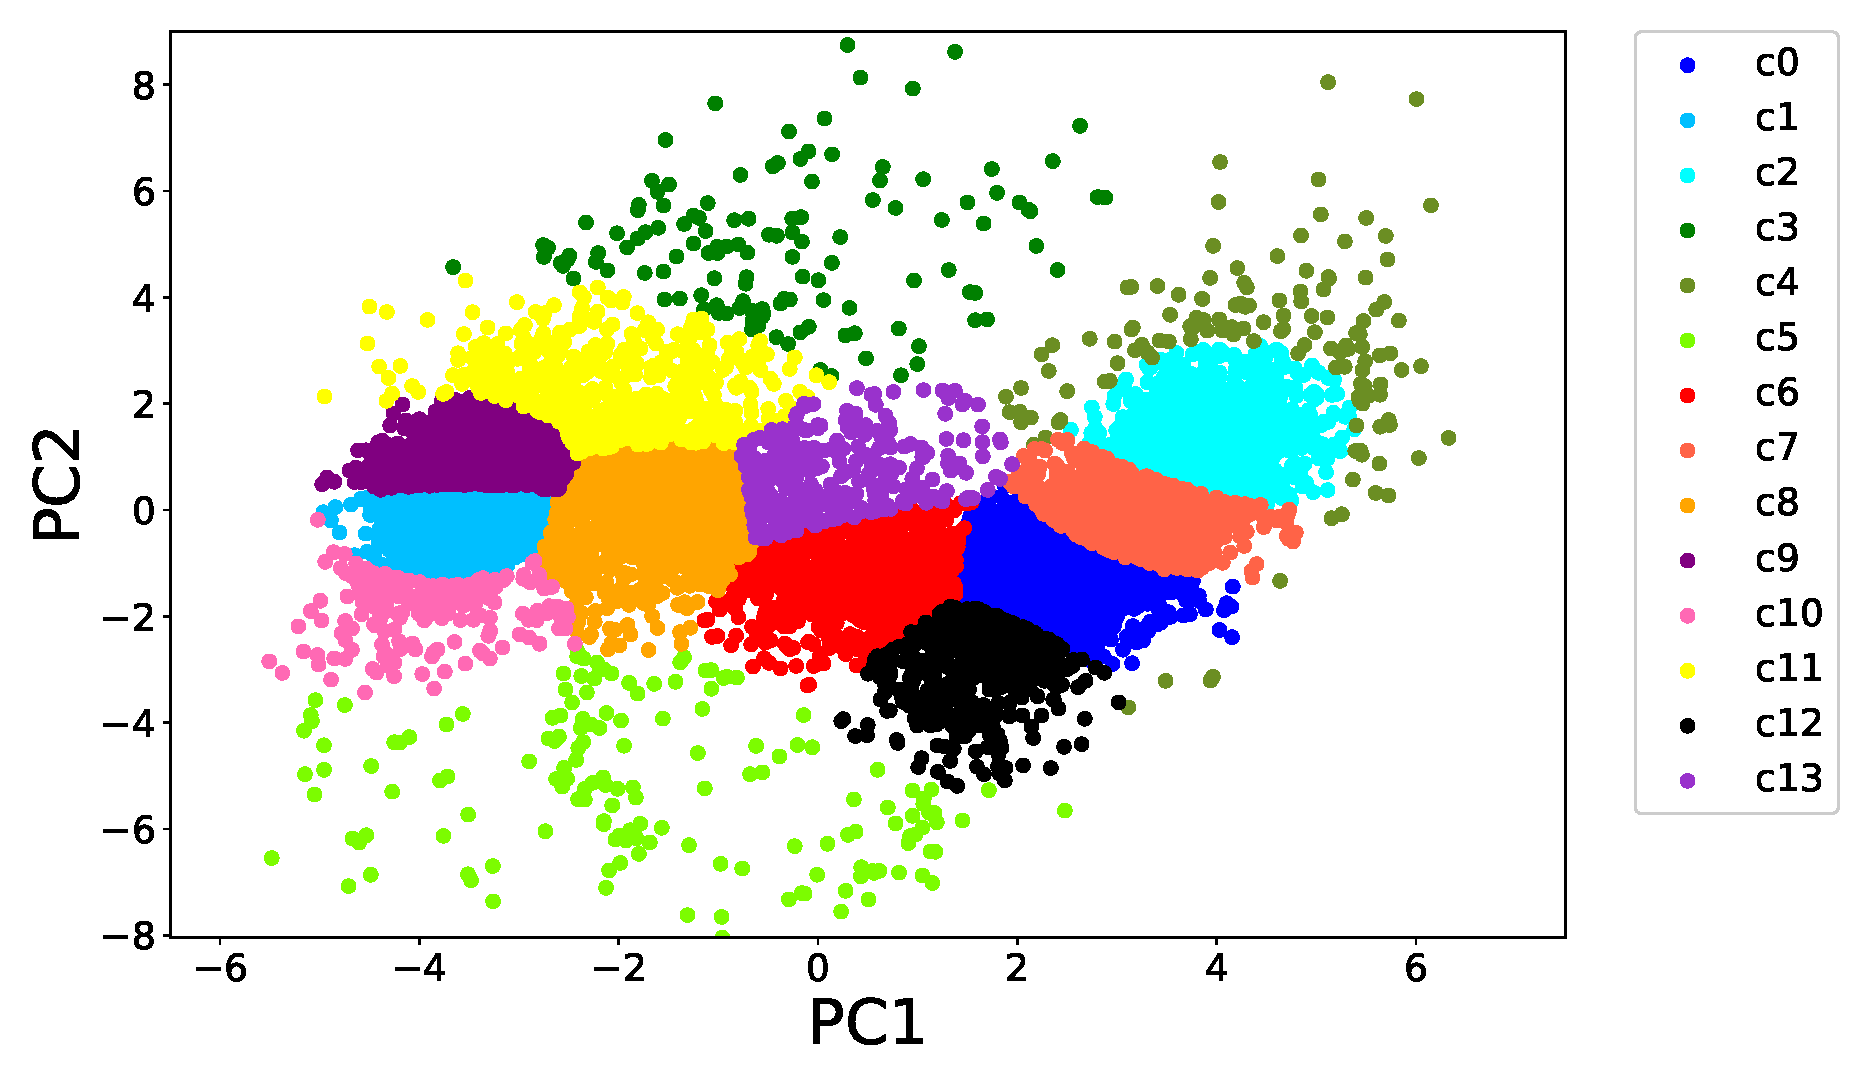
\includegraphics[width=\columnwidth]{images/fencing/gmm.eps}
    \caption{Clustering results. Up to the second principal component is illustrated.}
    \label{fig:gmm_result}
\end{figure}

As an example application of the skeletal information obtained by the proposed framework, clustering was performed.
The results of clustering up to the second principal component of the skeletal information with a mixed Gaussian model are shown in Figure \ref{fig:gmm_result}.
The legend indicates each cluster.
Some of the representative posture frames for each cluster are shown in Figure \ref{fig:eg_frame}.
A characteristic posture was observed in each cluster.
The most common posture observed in cluster c2 was the most neutral posture, which can be shifted to any posture.
Cluster c4, on the other hand, had a lower posture than the posture frames of the other clusters, with the epee sword sticking out in front of the body.
The posture of cluster c4 was lower than that of the other clusters, and it was considered to be an attacking posture, based on the characteristics of fencing.
Thus, clustering using the proposed framework may make it easier to classify the plays.
In addition, the posture frames of clusters c8 and c13 are not directly related to the play.
Clustering can also remove these data, which would otherwise have to be done manually.


\begin{figure}
\centering
\begin{tabular}{cccc}
\subfloat[c2]{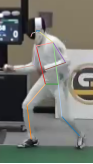
\includegraphics[height = 20mm]{images/fencing/normal.png}} &
\subfloat[c4]{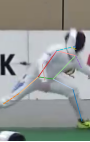
\includegraphics[height = 20mm]{images/fencing/attack.png}} &
%\subfloat[]{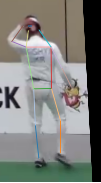
\includegraphics[height = 20mm]{images/fencing/ng2.png}} &
\subfloat[c8]{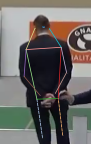
\includegraphics[height = 20mm]{images/fencing/ng3.png}} &
\subfloat[c13]{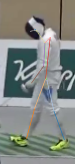
\includegraphics[height = 20mm]{images/fencing/ng1.png}}
\end{tabular}
%\caption{Visualization of the clusters created when clustering the frame-by-frame skeletal information using a mixed Gaussian distribution. (a), (b), (c), (d), and (e) are representative frames of each belonging cluster.}
\caption{An example of a cluster posture frame. The label is the same as in Figure \ref{fig:gmm_result}}.
\label{fig:eg_frame}
\end{figure}

\section{conclusion}
In this study, we proposed an analytical framework for extracting video and numeric values to assist experts in their analysis tasks using computer vision and machine learning in the epee fencing event.
As a future prospect, we will conduct a more rigorous evaluation of the proposed method and try to extend the framework to other events.

